%----------------------------------------------------------------------------------------
%	PACKAGES AND OTHER DOCUMENT CONFIGURATIONS
%----------------------------------------------------------------------------------------

\documentclass[11pt,twoside,twocolumn,russian,a4paper]{article}

\usepackage{blindtext} % Package to generate dummy text throughout this template 
\usepackage{graphicx}
\usepackage{bm}
\usepackage{amsmath}
\usepackage[sc]{mathpazo} % Use the Palatino font
\usepackage[T1,T2A]{fontenc} % Use 8-bit encoding that has 256 glyphs
\usepackage[utf8]{inputenc}
\linespread{1.05}         % Line spacing - Palatino needs more space between lines
%\usepackage{microtype}    % Slightly tweak font spacing for aesthetics

\usepackage[russian]{babel} % Language hyphenation and typographical rules

\usepackage[hmarginratio=1:1,top=32mm,bottom=32mm,left=25mm,right=25mm,columnsep=20pt]{geometry}  % Document margins
\usepackage[hang,small,labelfont=bf,up,textfont=it,up]{caption} % Custom captions under/above floats in tables or figures
\usepackage{booktabs} % Horizontal rules in tables

%usepackage{lettrine}        % The lettrine is the first enlarged letter at the beginning of the text
\usepackage{enumitem}        % Customized lists
\setlist[itemize]{noitemsep} % Make itemize lists more compact

\usepackage{abstract} % Allows abstract customization
\renewcommand{\abstractnamefont}{\normalfont\bfseries} % Set the "Abstract" text to bold
\renewcommand{\abstracttextfont}{\normalfont\small\itshape} % Set the abstract itself to small italic text

\usepackage{titlesec} % Allows customization of titles
\renewcommand\thesection{\Roman{section}} % Roman numerals for the sections
\renewcommand\thesubsection{\roman{subsection}} % roman numerals for subsections
\titleformat{\section}[block]{\large\scshape\centering}{\thesection.}{1em}{} % Change the look of the section titles
\titleformat{\subsection}[block]{\large}{\thesubsection.}{1em}{} % Change the look of the section titles

\usepackage{fancyhdr} % Headers and footers
\pagestyle{fancy}     % All pages have headers and footers
\fancyhead{}          % Blank out the default header
\fancyfoot{}          % Blank out the default footer
\fancyhead[C]{Моделирование колоний $\bullet$ Март 2018 $\bullet$ Курсовая работа} % Custom header text
\fancyfoot[CO,CE]{\thepage} % Custom footer text[RO,LE]

\usepackage{titling}        % Customizing the title section
\usepackage{hyperref}       % For hyperlinks in the PDF


%----------------------------------------------------------------------------------------
%	TITLE SECTION
%----------------------------------------------------------------------------------------

\setlength{\droptitle}{-5\baselineskip} % Move the title up

\pretitle{\begin{center}\huge\bfseries} % Article title formatting
\posttitle{\end{center}} % Article title closing formatting
\title{Моделирование популяции колонии микроорганизмов} % Article title
\author{
	\textsc{Ф. Сергеев, В. Аксёнов} \\[0.5ex] % Your name
	\normalsize 675гр. ФУПМ МФТИ \\ % Your institution
	\normalsize \href{mailto:sergeev.fi@phystech.edu}{sergeev.fi@phystech.edu}, \href{mailto:aksenov.vv@phystech.edu}{aksenov.vv@phystech.edu}	\normalsize 
}
\date{\today} % Leave empty to omit a date

\renewcommand{\maketitlehookd}{%
\begin{abstract}
\vspace{-0.5cm} \noindent  В процессе эволюции, с изменением генетического кода организмов, меняется и их поведение. В результате выживают организмы с более эффективным алгоритмом поведения. Цель данной работы состоит в моделировании процесса развития конкурирующих колоний микроорганизмов при условии ограниченности ресурсов.
\end{abstract}
}

%----------------------------------------------------------------------------------------

\graphicspath{ {/} }

\begin{document}

\maketitle

%----------------------------------------------------------------------------------------
%	ARTICLE CONTENTS
%----------------------------------------------------------------------------------------

\section{Модель}

\noindent Среда обитания микроорганизмов~---~двумерное поле $n\times m$. Бактерии за одну единицу времени могут переходить в соседнюю клетку по стороне или углу.  <  ВЗАИМОДЕЙСТВИЕ С ПИЩЕЙ И ДРУГ ДРУГОМ >

\section{Приложение}

\noindent Предлагается визуализировать процесс развития колоний в реальном времени, с возможностью паузы/возобновления процесса, а также возможность сохранения/импортирования данных. \smallskip\\
\noindent В левой части окна находится двумерное поле, собственно представляющее среду обитания колоний. Отдельные микроорганизмами обозначены синим (первая колонии), и зелёным (вторая колония) цветом соответственно. Источники пищи обозначены жёлтым цветом. Постоянные источники пищи~---~жёлтым цветом и буквой <<И>>. Пустое поле обозначается белым цветом.\smallskip

\begin{figure}[h]
	\centering
	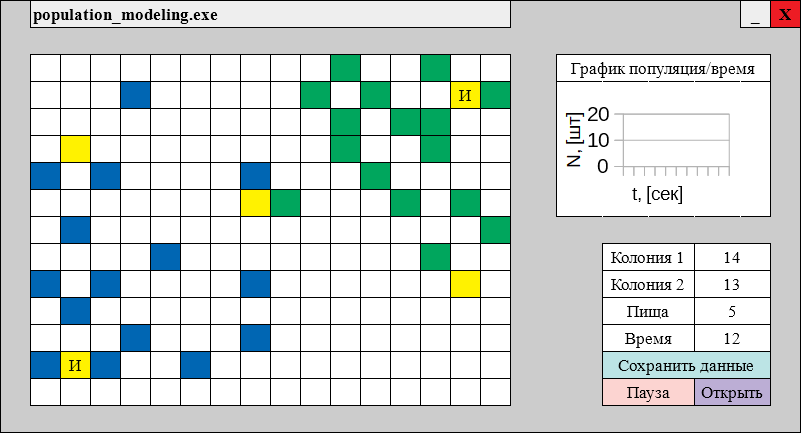
\includegraphics[width=0.45\textwidth]{scheme_big}
	\caption{Макет оконного приложения}
\end{figure}

\noindent В правой части окна представлены данные протекающего эксперимента: вверху~---~график зависимости количества особей обеих колоний (и, возможно, доступной пищи) от времени, посередине~---~численные данные (текущее количество особей обоих колоний, текущее количество единиц пищи, время, прошедшее с начала эксперимента), внизу~---~кнопки для сохранения данных об эксперименте, паузы/возобновления эксперимента, и импорта параметров сохранённого эксперимента.\smallskip\\
\noindent Дополнительный функционал:
\begin{itemize}
	\item Возможность ускорения/замедления времени.
	\item Интерактивное добавление пищи с помощью мыши.
	\item <<Стенки>>~---~ограничение движения бактерий.
\end{itemize}

\section{Эволюционное развитие$^*$}
\noindent В качестве дополнительной задачи предлагается построить и имплементировать механизм <<мутаций>>. Если поведение бактерии задаётся некоторым набором команд (движение, реакция на пищу, реакция на бактерию из конкурирующей колонии и.~т.~д.), то некоторое произвольное изменение этого набора приведёт к изменению поведения бактерии. Будем запускать эксперимент на некоторое определённое время, в конце выбирая несколько доминирующих колоний. Далее <<мутируем>> алгоритм их поведения и повторяем процедуру отбора. Таким образом построена модель <<естественного>> отбора эволюционирующих особей.\smallskip\\
\noindent Формулировка данной дополнительной задачи не окончательна и будет дорабатываться по ходу работы над проектом.

%----------------------------------------------------------------------------------------
%	REFERENCE LIST
%----------------------------------------------------------------------------------------

\bibliographystyle{plain}
\begin{thebibliography}{99}

\bibitem{veksler} В. И. Ленин.  Полное собрание трудов, т. 22 // Доклады АН СССР. -- 1944. -- Т. 43, № 8. -- С. 346-348.
 
\end{thebibliography}

%----------------------------------------------------------------------------------------

\end{document}
